\begin{question}{27}{
    Een onderzoekseenheid van Damen Naval voert een analyse uit op de relatie tussen de snelheid van een marinefregat (in knopen) en haar akoestische signatuur (in decibel).
    Hiervoor worden $11$ fregatten aselect gekozen en worden de volgende metingen verricht: 
    {\footnotesize
        \begin{center}
            \begin{tabular}{c|ccccccccccc}
                \toprule
                    \multilinecell{\textbf{Snelheid} \\ \textbf{(knopen)}} & $8.0$ & $10.0$ & $12.0$ & $14.0$ & $16.0$ & $18.0$ & $20.0$ & $22.0$ & $24.0$ & $26.0$ & $28.0$ \\
                \midrule
                    \multilinecell{\textbf{Akoestische} \\ \textbf{signatuur (dB)}} & $116.7$ & $124.0$ & $123.3$ & $123.5$ & $120.6$ & $122.1$ & $122.6$ & $132.2$ & $131.0$ & $133.6$ & $128.2$ \\
                \bottomrule
            \end{tabular}
        \end{center}
    }
}
    
    \subquestion{2}{
        Als we een regressie-analyse willen uitvoeren, welke variabele zou dan de afhankelijke variabele $Y$ zijn en welke variabele zou de onafhankelijke variabele $X$ zijn?
    }
    \solution{
        Bij een regressie-analyse is de meest logische keuze om snelheid als onafhankelijke variabele $X$ te kiezen, en de akoestische signatuur als afhankelijke variabele $Y$. 
        Een hogere akoestische signatuur verklaart niet de snelheid van een fregat, terwijl dat andersom wellicht wel het geval kan zijn.\rubric{2}
    }
    \subquestion{4}{
        Teken het bijbehorende spreidingsdiagram op basis van je antwoord op vraag a.
        Geef hierbij duidelijk aan welke as welke variabele voorstelt.
    }
    \solution{
        Het spreidingsdiagram is hieronder weergegeven, waarbij de kruissnelheid (in knopen) op de $x$-as is uitgezet en de akoestische signatuur (in decibel) op de $y$-as.\rubric{2}
        \begin{center}
            \resizebox{0.9\textwidth}{!}{
                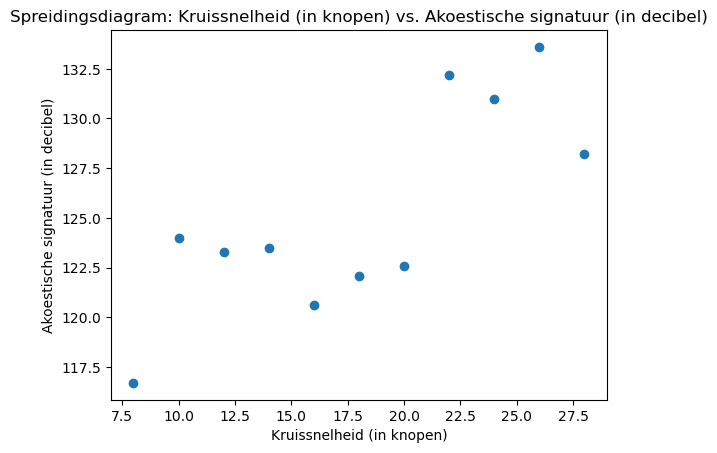
\includegraphics{20251113_scatterplot.png} 
            }
        \end{center}\rubric{2}
    }

    \subquestion{7}{
        Bereken Pearson's correlatieco\"effici\"ent $r(x,y)$ op basis van de data in de bovenstaande tabel.
        Wat zegt $r(x, y)$ over de relatie tussen snelheid en akoestische signatuur?
    }
    \solution{
        We beginnen met het uitrekenen van Pearson's correlatieco\"effici\"ent 
        \begin{align*}
            r(x,y)  &= \frac{ \overline{x \cdot y} - \overline{x} \cdot \overline{y} }{ \sqrt{ (\overline{x^2} - \overline{x}^2 ) \cdot (\overline{y^2} - \overline{y}^2) }}
        \end{align*}
        Hiervoor hebben we dus de waardes van $\overline{x}$, $\overline{y}$, $\overline{xy}$, $\overline{x^2}$ en $\overline{y^2}$ nodig.
        Deze bepalen we aan de hand van de volgende rekentabel:
        \begin{center}
            \begin{tabular}{ccccc}
                \toprule
                    $x$ & $y$ & $xy$ & $x^2$ & $y^2$ \\
                \midrule
                    $8$ & $116.7$ & $933.6$ & $64$ & $13618.89$ \\
                    $10$ & $124$ & $1240$ & $100$ & $15376$ \\
                    $12$ & $123.3$ & $1479.6$ & $144$ & $15202.89$ \\
                    $14$ & $123.5$ & $1729$ & $196$ & $15252.25$ \\
                    $16$ & $120.6$ & $1929.6$ & $256$ & $14544.36$ \\
                    $18$ & $122.1$ & $2197.8$ & $324$ & $14908.41$ \\
                    $20$ & $122.6$ & $2452$ & $400$ & $15030.76$ \\
                    $22$ & $132.2$ & $2908.4$ & $484$ & $17476.84$ \\
                    $24$ & $131$ & $3144$ & $576$ & $17161$ \\
                    $26$ & $133.6$ & $3473.6$ & $676$ & $17848.96$ \\
                    $28$ & $128.2$ & $3589.6$ & $784$ & $16435.24$ \\
                \midrule
                    $\overline{x} = 18$ & $\overline{y} = 125.2545$ & $\overline{xy} = 2279.7455$ & $\overline{x^2} = 364$ & $\overline{y^2} = 15714.1455$ \rubric{3} \\
                \bottomrule
            \end{tabular}
        \end{center}

        De correlatieco\"effici\"ent van Pearson is dus gelijk aan
        \begin{align*}
            r(x,y)  &= \frac{ \overline{x \cdot y} - \overline{x} \cdot \overline{y} }{ \sqrt{ (\overline{x^2} - \overline{x}^2) \cdot (\overline{y^2} - \overline{y}^2) } }\\
                    &= \frac{ 2279.7455 - 18 \cdot 125.2545 }{ \sqrt{ (364 - 18^2) \cdot (15714.1455 - 125.2545^2) } } \\
                    &= \frac{25.1636}{31.9025} \\
                    &\approx 0.7888. \rubric{2}
        \end{align*}
        De correlatieco\"effici\"ent $r \approx 0.7888$ ligt ver van $0$ af en is positief.
        Dit houdt in dat er een vrij sterke positieve (stijgende) trend is. \rubric{1}
        Een hogere snelheid van het fregat correleert met een hogere akoestische signatuur. \rubric{1}
    }

    \subquestion{6}{
        Bereken de regressielijn $Y = a + b \cdot X$ door berekening van de co\"effici\"enten $a$ en $b$.
        Bepaal aan de hand van de regressielijn een statistisch verantwoorde voorspelling voor de akoestische signatuur van een fregat dat $11.2$ knopen vaart.
    }
    \solution{
        Om de co\"effici\"enten $a$ en $b$ van de regressielijn te berekenen, gaan we de rekentabel van vraag (a) hergebruiken.
        Er volgt namelijk dat
        \begin{align*}
            b &= \frac{\overline{xy} - \overline{x} \cdot \overline{y}}{\overline{x^2} - (\overline{x})^2} \\
              &= \frac{2279.7455 - 18 \cdot 125.2545}{364 - (18)^2} \\
              &= \frac{25.1636}{40} \approx 0.6291 \\ \rubric{2}
            a &= \overline{y} - b \cdot \overline{x} \\
              &= 125.2545 - 0.6291 \cdot 18 \\
              &\approx 113.9309. \rubric{2}
        \end{align*}
        De formule van de regressielijn behorende bij deze steekproef is dus gelijk aan $Y = 113.9309+0.6291X$. \rubric{1}
        Een statistisch verantwoorde voorspelling voor de akoestische signatuur van een fregat dat $11.2$ knopen vaart vinden we door $X = 6.75$ in te vullen:
        Dit geeft een waarde van $Y = 113.9309 + 0.6291 \cdot 11.2 \approx 120.9767$, oftewel net iets minder dan $121$ decibel. \rubric{1} 
    }

    \subquestion{8}{
        Bereken een \SI{95}{\percent}-betrouwbaarheidsinterval voor de gemiddelde akoestische signatuur van fregatten die met een kruissnelheid van $11.2$ knopen varen.
        Rond af op gehele getallen zodanig dat het betrouwbaarheidsniveau gewaarborgd blijft.
    }
    \solution{
        In opdracht (d) hebben we een puntschatting van $y_0 = 113.9309 + 0.6291 \cdot 11.2 \approx 120.9767$ bepaald.
        Daarnaast kunnen we de standaardafwijking $\sigma$ van de storingsterm $\varepsilon$ schatten:
        \begin{align*}
            s_{\varepsilon} &= \sqrt{ \frac{n}{n-2} \cdot \left( \overline{y^2} - a \cdot \overline{y} - b \cdot \overline{xy} \right) } \\ 
                            &= \sqrt{ \frac{11}{9} \cdot \left( 15714.1455 - 113.9309 \cdot 125.2545 - 0.6291 \cdot 2279.7455 \right) } \\ 
                            &\approx 3.4279. \rubric{2}
        \end{align*}

        Vervolgens kunnen we een puntschatting berekenen van de standaardafwijking van $Y$ voor gegeven $X = x_0$:
        \begin{align*}
        s_{\mu}  &= s_{\varepsilon} \cdot \sqrt{ \frac{1}{n} \cdot \left( 1 + \frac{(x_0 - \overline{x})^2}{\overline{x^2} - \overline{x}^2} \right) } \\
                    &= 3.4279 \cdot \sqrt{ \frac{1}{11} \cdot \left( 1 + \frac{(11.2 - 18)^2}{364 - 18^2} \right) } \\
                    &\approx 1.5176. \rubric{2}
        \end{align*}

        Omdat we de standaardafwijkingen geschat hebben en de storingstermen normaal verdeeld zijn, moeten we werken met de $t$-verdeling met $df = n - 2 = 9$ vrijheidsgraden.
        De $t$-waarde die hoort bij een betrouwbaarheidsniveau $\alpha = 0.05$ is gelijk aan
        \[
            t = \invt(\text{opp} = 1 - \alpha / 2; \text{df} = n - 2) = \invt(\text{opp} = 0.975; \text{df} = 9) \approx 2.2622.\rubric{1}
        \]
        Het \SI{95}{\percent}-betrouwbaarheidsinterval voor de gemiddelde $Y$ voor gegeven $X = x_0$ kan dus worden beschreven door
        \begin{align*}
            &[y_0 - t \cdot s_{\mu}; y_0 - t \cdot s_{\mu}] \\
            &= [120.9767 - 2.2622 \cdot 1.5176; 120.9767 + 2.2622 \cdot 1.5176] \\
            &\approx [117.5437; 124.4098].\rubric{2}
        \end{align*}
        
        Met \SI{95}{\percent} zekerheid zal de gemiddelde akoestische signatuur van fregatten die met een kruissnelheid van $11.2$ knopen varen 
        tussen ongeveer 
        $117$ en $125$ decibel liggen (naar buiten afronden op betrouwbaarheidsniveau te waarborgen).\rubric{1} 
    }
\end{question}